%!TeX root=MemoriaTFG.tex

\chapter{Pipeline de construcción y caracterización del dataset DermapixelAI 1.0}
\label{anexo:pipeline}
\label{cap:anexoc}

Este anexo documenta el pipeline de construcción y la caracterización
cuantitativa completa del dataset DermapixelAI 1.0, descrito de forma
resumida en la sección~\ref{sec:datos} del
capítulo~\ref{cap:metodos}. El dataset se desarrolla en paralelo al
trabajo experimental del TFG, en el marco de la modernización
tecnológica del archivo Dermapixel introducida en el
capítulo~\ref{cap:intro}, y se publica como contribución
independiente del trabajo a la comunidad investigadora.

\section{Origen y materia prima}
\label{sec:anexo-origen}

El dataset DermapixelAI se construye a partir del archivo del blog
Dermapixel. La materia prima es el conjunto de casos publicados
durante más de quince años por la Dra.~R.~Taberner, cada uno
acompañado de imágenes (fotografía clínica y, cuando procede, imagen
dermatoscópica), historia clínica abreviada en castellano y
diagnóstico final con razonamiento.

\section{Pipeline de construcción}
\label{sec:anexo-pipeline}

La construcción del dataset se desarrolla como un proceso iterativo,
ajustado en sucesivas revisiones internas en función de las
auditorías de integridad realizadas sobre el dataset, hasta consolidar
la versión 1.0 documentada en este anexo como primera versión estable
y publicable. El pipeline final se compone de seis pasos.

\paragraph{(i) Extracción.} Recogida de las publicaciones del blog y
de los metadatos asociados por caso (título, fecha, texto narrativo,
imágenes, diagnóstico final). El proceso se ejecuta con scripts
deterministas a partir de la fuente HTML del blog.

\paragraph{(ii) Deduplicación.} Cálculo de hash MD5 sobre cada imagen
y eliminación de duplicados exactos. Identificación de imágenes
asociadas a la pista de solución de los casos del blog ---imágenes
que aparecen sólo en la entrada del solucionario y que llevan
información asociada al diagnóstico final, susceptibles de inducir
\emph{leakage} si se incluyen--- y su exclusión documentada.

\paragraph{(iii) Clasificación de modalidad.} Asignación a cada
imagen de su modalidad (\emph{clinical}, \emph{dermoscopy},
\emph{histology}, \emph{ultrasound} o \emph{wood\_lamp}) mediante una
combinación de heurísticas sobre el nombre del fichero y revisión
manual de los casos no resueltos automáticamente con confianza
suficiente. El paso incluye una auditoría sistemática sobre la
totalidad del dataset para detectar y corregir asignaciones erróneas,
así como la exclusión de imágenes que tras la revisión visual
resultan no ser contenido dermatológico (banners institucionales,
ilustraciones, fotografías de eventos o material de archivo que
pudiera haber entrado al dataset por el scraping inicial); estas
últimas se trasladan a una carpeta \texttt{images/\_excluded/} y se
eliminan del fichero maestro \texttt{dataset.csv}, manteniéndose en
\texttt{cases.csv} con \texttt{num\_images\_in\_dataset = 0} cuando
el caso resulta sin imágenes tras la exclusión.

\paragraph{(iv) Mapeo ontológico.} Cada caso publicado contiene una
etiqueta diagnóstica generada por revisión textual del título y del
razonamiento. Esta etiqueta cruda se mapea, mediante revisión experta
de la Dra.~Taberner sobre la totalidad del dataset, a una entrada L3
de la ontología jerárquica descrita en la sección~\ref{sec:ontologia}
del capítulo~\ref{cap:metodos}. La revisión genera tres campos
asociados a cada imagen: \texttt{label\_source} (origen de la
etiqueta diagnóstica final), \texttt{diagnosis\_source} (origen del
razonamiento textual asociado al diagnóstico) y
\texttt{rosa\_verified} (validación visual de la imagen como caso
representativo del diagnóstico asignado).

\paragraph{(v) Particionado.} Asignación de cada imagen a uno de los
tres splits (\texttt{train}, \texttt{val}, \texttt{test}) bajo regla
de agrupamiento por caso (\emph{case-aware split}): todas las
imágenes de un mismo caso clínico van al mismo split, lo que previene
la fuga de información entre conjuntos.

\paragraph{(vi) Auditoría de integridad.} Verificación final de
hashes MD5, ausencia de imágenes corruptas, consistencia entre la
estructura de carpetas y \texttt{dataset.csv}, y ausencia de
referencias a imágenes inexistentes en disco. Todas las
modificaciones intermedias del dataset se acompañan de \emph{backup} y
registro de auditoría (\texttt{audit\_log.txt} y
\texttt{excluded\_images.csv}) para preservar trazabilidad histórica.

La versión 1.0 del dataset, consolidada como resultado de este
pipeline, contiene 1\,089 imágenes vinculadas a 669 casos
clínicos con identificador único resoluble, sobre un total de
698 casos catalogados en el archivo original (de los cuales 672
disponen de imagen efectiva antes de la deduplicación MD5; los
tres casos restantes se pierden por duplicado exacto de imagen
entre entradas distintas del blog).

\section{Cardinalidades del dataset y splits experimentales}
\label{sec:anexo-cardinalidades}

A lo largo del trabajo coexisten tres particiones distintas del
dataset, todas derivadas del mismo pipeline pero filtradas con
criterios específicos según el experimento. La
tabla~\ref{tab:anexo-cardinalidades} resume las cardinalidades para
evitar confusión entre referencias cruzadas.

\begin{table}[H]
\centering
\small
\caption{Cardinalidades del dataset DermapixelAI~1.0 según
configuración. Los splits son \emph{case-aware} (ningún caso se
reparte entre splits). El test del estudio principal sobre el
dataset de producción es deliberadamente reducido para reservar
masa de validación interna a la futura cohorte prospectiva del
HUSLL (Sección~\ref{sec:linea-prospectivo}).}
\label{tab:anexo-cardinalidades}
\begin{tabular}{p{0.21\textwidth}rrrr p{0.30\textwidth}}
\hline
Configuración & Imágenes & Casos & Train & Val/Test & Uso \\
\hline
Producción (\texttt{dataset.csv})           & 1\,089 & 669 & 891 & 157 / 41 & Estudio principal del Capítulo~\ref{cap:resultados} \\
Filtrada (\texttt{dataset\_filtered.csv})   & 1\,062 & 653 & 874 & 152 / 36 & Restricción a \emph{clinical+dermoscopy} con \texttt{label\_source=ontology} \\
Dermapixel R0 contrastivo (Sec.~\ref{sec:spanderm-clip}) & 1\,062 & 653 & 854 & 107 / 101 & Experimento dual-encoder con \emph{manifest} SHA-256 propio \\
\hline
\end{tabular}
\end{table}

Las tres configuraciones comparten el archivo subyacente y la
regla de partición case-aware, pero aplican filtros y \emph{seeds}
distintos. La cifra base $1\,089$ es el resultado del pipeline
completo; el subconjunto filtrado de $1\,062$ excluye 27 imágenes
que pierden trazabilidad ontológica tras la auditoría de mapeo; y
los splits de la rama contrastiva de Dermapixel R0 de $854/107/101$ son reproducibles a
partir del \emph{manifest} SHA-256 pinned en cada checkpoint del
experimento (Sección~\ref{sec:spanderm-clip}).

\section{Distribución por modalidad}
\label{sec:anexo-modalidad}

La tabla~\ref{tab:anexo-modalidad} resume la composición del dataset
por modalidad.

\begin{table}[H]
\centering
\small
\caption{Distribución del dataset DermapixelAI 1.0 por modalidad de
imagen.}
\label{tab:anexo-modalidad}
\begin{tabular}{lr}
\hline
Modalidad        & N       \\
\hline
clinical         & 1\,036  \\
dermoscopy       & 49      \\
histology        & 2       \\
ultrasound       & 1       \\
wood\_lamp       & 1       \\
\hline
\textbf{Total en \texttt{dataset.csv}} & \textbf{1\,089} \\
\hline
\end{tabular}
\end{table}

La fotografía clínica predomina con claridad sobre el resto de
modalidades. El subconjunto dermatoscópico, con 49 imágenes,
constituye un grupo reducido pero suficiente para análisis
exploratorios específicos sobre esa modalidad.

\section{Distribución por categoría etiológica L1}
\label{sec:anexo-l1}

La distribución por L1 (tabla~\ref{tab:anexo-l1}) muestra el
predominio de la patología inflamatoria, seguida por las patologías
tumoral e infecciosa con pesos similares y un porcentaje residual de
genodermatosis.

\begin{table}[H]
\centering
\small
\caption{Distribución del dataset DermapixelAI 1.0 por categoría
etiológica L1. La fila ``(sin asignar)'' recoge las 19 imágenes cuyo
mapeo ontológico no se ha completado (todas ellas corresponden a
casos con \texttt{label\_source = raw}).}
\label{tab:anexo-l1}
\begin{tabular}{lrr}
\hline
Categoría L1               & N       & \%      \\
\hline
Patología inflamatoria     & 544     & 49,9    \\
Patología tumoral          & 276     & 25,3    \\
Patología infecciosa       & 259     & 23,8    \\
Genodermatosis             & 11      & 1,0     \\
(sin asignar)              & 19      & ---     \\
\hline
\textbf{Total}             & \textbf{1\,089} & \textbf{100,0} \\
\hline
\end{tabular}
\end{table}

\section{Distribución por subcategoría L2 y por diagnóstico L3}
\label{sec:anexo-l2-l3}

La figura~\ref{fig:eda-l1} ilustra la distribución L1 etiológica
sobre el subconjunto filtrado (clinical + dermoscopy, con
\texttt{label\_source = ontology} y L1 asignada), utilizado en la
caracterización del dataset efectivo. Patología inflamatoria
concentra la mitad del dataset, mientras que Genodermatosis ocupa la
cola corta con sólo $8$ imágenes ($0{,}8$\%), lo que explica su
ausencia en el split de \texttt{test}.

\begin{figure}[H]
\centering
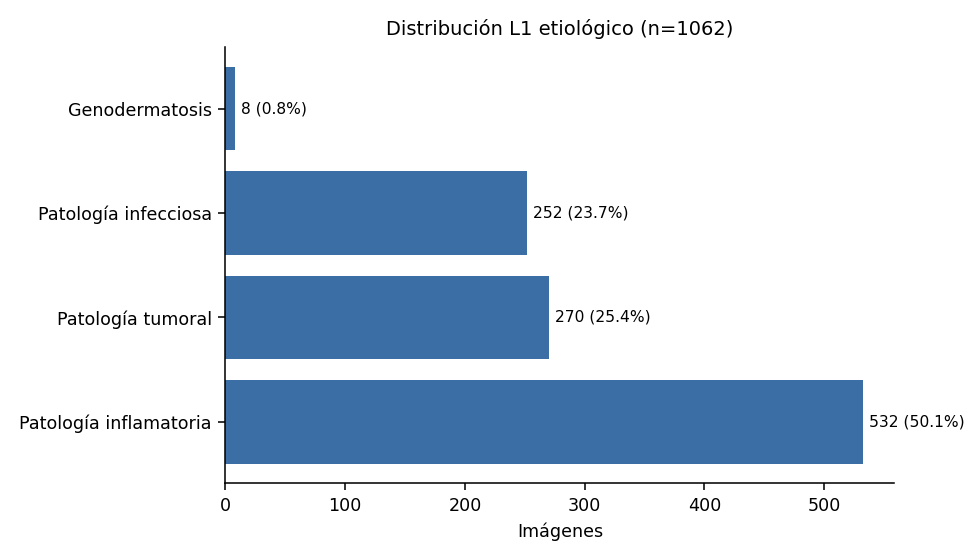
\includegraphics[width=0.85\textwidth]{figures/fig_eda_l1.png}
\caption{Distribución L1 etiológica sobre las $1\,062$ imágenes
filtradas. Patología inflamatoria concentra el $50{,}1$\%;
Genodermatosis es la cola corta con $8$ imágenes ($0{,}8$\%).}
\label{fig:eda-l1}
\end{figure}

De las 43 entradas L2 del vocabulario, 38 aparecen representadas en
el dataset DermapixelAI 1.0 con al menos una imagen. La cifra
observada en la extracción inicial es 39, pero dos de esas 39
corresponden a variantes ortográficas de la misma subcategoría
(\emph{Trastornos de la queratinización} y \emph{Trastornos
queratinización}); la normalización pendiente reduce la cifra
efectiva a 38. La figura~\ref{fig:eda-l2} muestra las veinte
subcategorías L2 más representadas.

\begin{figure}[H]
\centering
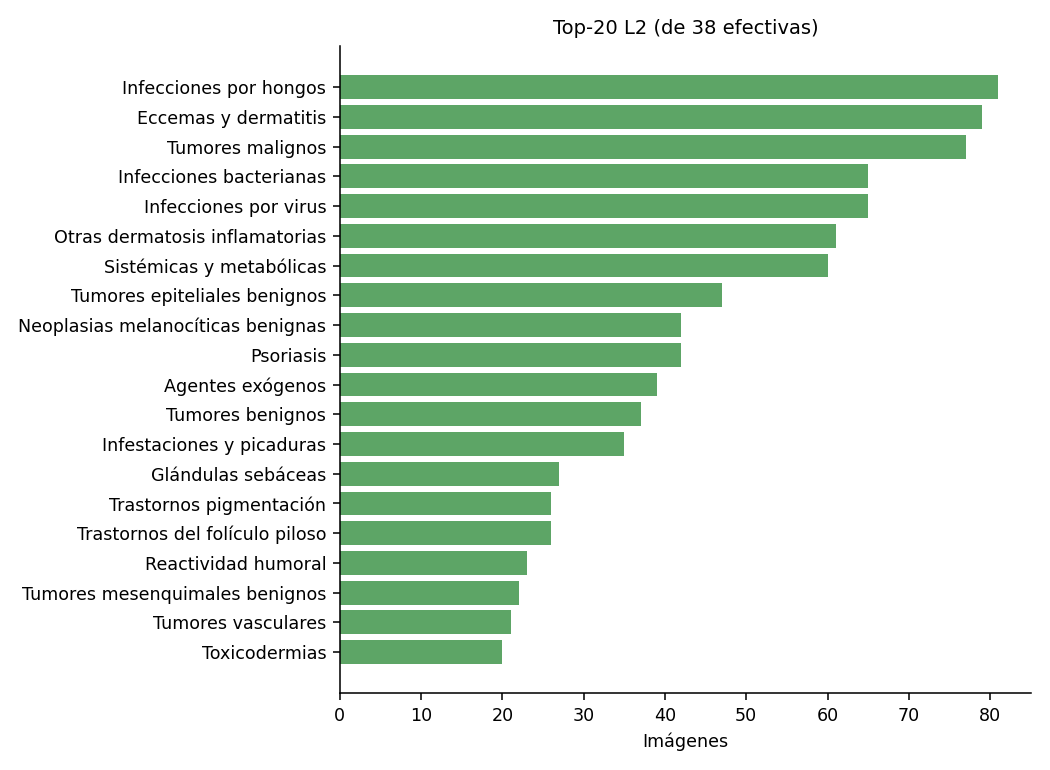
\includegraphics[width=0.95\textwidth]{figures/fig_eda_l2.png}
\caption{Top-20 subcategorías L2 sobre las 38 efectivamente
representadas en el dataset, ordenadas por número de imágenes.}
\label{fig:eda-l2}
\end{figure}

A nivel L3, 250 entradas del vocabulario están representadas en el
dataset, sobre las 367 entradas declaradas (cobertura efectiva del
68,1\%). El diagnóstico L3 más frecuente en el dataset es
\emph{Psoriasis en placas} (38 imágenes), seguido por \emph{Tiña
corporis} (32), \emph{Liquen plano} (28) y \emph{Nevo melanocítico
adquirido} (25). Los veinte L3 más representados concentran
aproximadamente el 32\% del dataset.

La tabla~\ref{tab:anexo-top10-l3} recoge los diez diagnósticos L3 con
mayor número de imágenes en el dataset. Estos diez diagnósticos
concentran $234$ imágenes, equivalentes al $22{,}0$\% del dataset
filtrado.

\begin{table}[H]
\centering
\small
\caption{Top-10 diagnósticos L3 más frecuentes en el dataset
DermapixelAI 1.0.}
\label{tab:anexo-top10-l3}
\begin{tabular}{lr}
\hline
Diagnóstico L3                          & N    \\
\hline
Psoriasis en placas                     & 38   \\
Tiña corporis                           & 32   \\
Liquen plano                            & 28   \\
Nevo melanocítico adquirido             & 25   \\
Carcinoma basocelular                   & 23   \\
Queratosis actínica                     & 21   \\
Dermatitis alérgica de contacto         & 21   \\
Acné                                    & 16   \\
Dermatofibroma                          & 16   \\
Melanoma                                & 14   \\
\hline
\textbf{Total top-10}                   & \textbf{234} \\
\hline
\end{tabular}
\end{table}

\section{Cola larga diagnóstica}
\label{sec:anexo-long-tail}

La distribución por L3 presenta una cola larga pronunciada
(figura~\ref{fig:eda-l3-rank}). La
tabla~\ref{tab:anexo-cola-larga} cuantifica el reparto de las 250
clases L3 efectivamente representadas en el dataset según el número
de imágenes asociadas a cada clase.

\begin{table}[H]
\centering
\footnotesize
\caption{Cola larga L3 sobre las 250 clases efectivas del dataset
DermapixelAI 1.0.}
\label{tab:anexo-cola-larga}
\begin{tabular}{lrr}
\hline
Rango imgs/clase & N\textsuperscript{o} clases L3 & \% del total \\
\hline
1 img       & 64  & 25,6  \\
2--5 imgs   & 129 & 51,6  \\
6--10 imgs  & 39  & 15,6  \\
11--20 imgs & 11  & 4,4   \\
21+ imgs    & 7   & 2,8   \\
\hline
\textbf{Total} & \textbf{250} & \textbf{100,0} \\
\hline
\end{tabular}
\end{table}

El $77{,}2$\% de las 250 clases L3 efectivamente representadas
dispone de cinco imágenes o menos, y un cuarto del total ($25{,}6$\%)
cuenta con una única imagen (figura~\ref{fig:eda-l3-cola}). Esta característica condiciona la
viabilidad de un clasificador con cabeza directa a 250 clases L3 y
justifica la estrategia operativa de cabeza L2 con ranking L3 por
prototipos descrita en la
sección~\ref{sec:lineas-abiertas} del capítulo~\ref{cap:conclusiones}.

\begin{figure}[H]
\centering
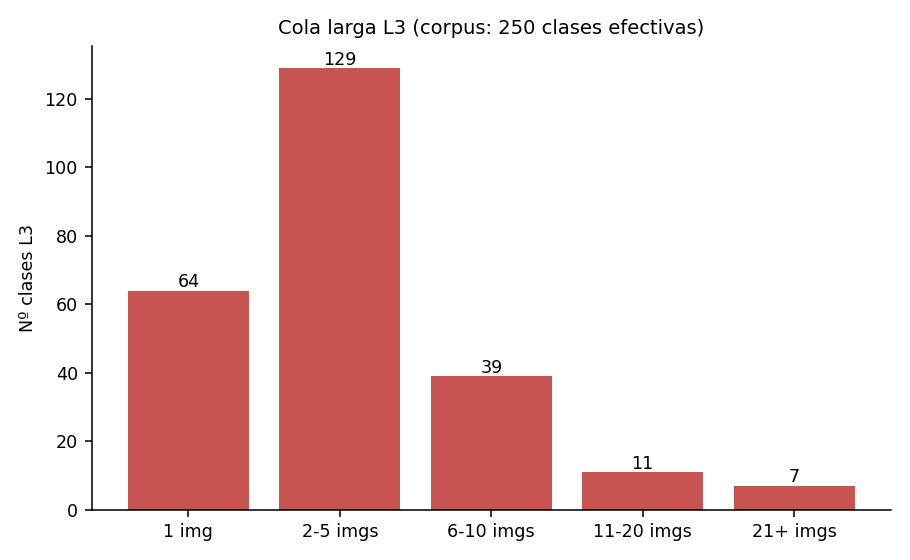
\includegraphics[width=0.85\textwidth]{figures/fig_eda_l3_cola.png}
\caption{Distribución de las 250 clases L3 efectivas en los cinco
rangos definidos en la tabla~\ref{tab:anexo-cola-larga}. Las clases
con cinco imágenes o menos suman el $77{,}2$\% del total.}
\label{fig:eda-l3-cola}
\end{figure}

\begin{figure}[H]
\centering
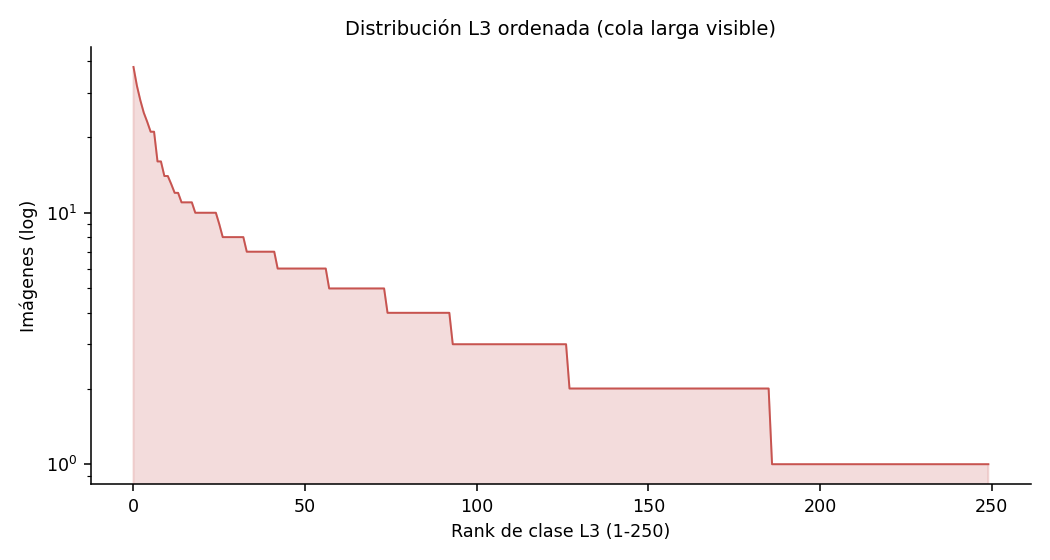
\includegraphics[width=0.95\textwidth]{figures/fig_eda_l3_rank.png}
\caption{Distribución rankeada del número de imágenes por clase L3
(eje vertical en escala logarítmica). El perfil decae rápidamente
tras los diez diagnósticos más frecuentes, lo que evidencia la
asimetría de la cola larga diagnóstica.}
\label{fig:eda-l3-rank}
\end{figure}

\section{Particionado en train, validación y test}
\label{sec:anexo-splits}

El dataset asigna sus splits bajo regla \emph{case-aware}: cada caso
clínico, identificado por \texttt{case\_id}, está íntegro en un único
split. La figura~\ref{fig:eda-casos} resume cuántas imágenes aporta
cada caso (media $1{,}63$, mediana $2$, máximo $5$).

\begin{table}[H]
\centering
\small
\caption{Tamaño de los splits oficiales del dataset DermapixelAI 1.0
con regla case-aware (cada caso clínico íntegro en un único split).}
\label{tab:anexo-splits}
\begin{tabular}{lr}
\hline
Split & N \\
\hline
train & 891 \\
val   & 157 \\
test  & 41  \\
\hline
\textbf{Total} & \textbf{1\,089} \\
\hline
\end{tabular}
\end{table}

La regla \emph{case-aware} se mantiene íntegra: ningún
\texttt{case\_id} aparece en más de un split. La verificación
explícita figura en el reporte de auditoría asociado al dataset.

La composición L1 dentro de cada split no es perfectamente
estratificada. En particular, Genodermatosis carece de representación
en \texttt{test} (las once imágenes de esta categoría se reparten
entre \texttt{train} y \texttt{val}), y once entradas L2 carecen de
imágenes en \texttt{val}, mientras que veintidós L2 carecen de
imágenes en \texttt{test}. Estos huecos limitan la granularidad de la
evaluación por L2 o por L1 sobre los splits oficiales
(figura~\ref{fig:eda-splits}).

\begin{figure}[H]
\centering
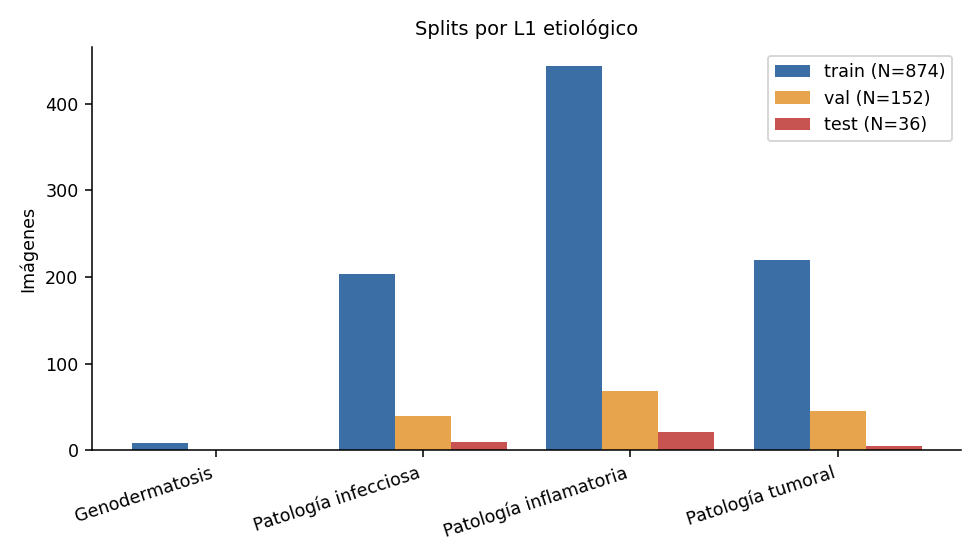
\includegraphics[width=0.85\textwidth]{figures/fig_eda_splits.png}
\caption{Balance L1 por split (\texttt{train}, \texttt{val},
\texttt{test}) sobre el subconjunto filtrado. Genodermatosis no
aparece en \texttt{test}.}
\label{fig:eda-splits}
\end{figure}

La tabla~\ref{tab:anexo-splits-niveles} desagrega el número de
imágenes, casos y entradas ontológicas únicas por nivel observadas
en cada split sobre el subconjunto filtrado utilizado para la
evaluación (clinical + dermoscopy con \texttt{label\_source =
ontology} y L1 asignada). Las cifras sobre el dataset completo
(1\,089 imágenes) son las de la tabla~\ref{tab:anexo-splits}.

\begin{table}[H]
\centering
\small
\caption{Cobertura ontológica por split sobre el subconjunto filtrado
(1\,062 imágenes). N\textsuperscript{o} de entradas únicas observadas
en cada nivel.}
\label{tab:anexo-splits-niveles}
\begin{tabular}{lrrrrr}
\hline
Split  & Imágenes & Casos & L1 & L2 & L3  \\
\hline
train  & 874      & 527   & 4  & 38 & 224 \\
val    & 152      & 98    & 3  & 28 & 72  \\
test   & 36       & 28    & 3  & 17 & 27  \\
\hline
\end{tabular}
\end{table}

El tamaño del split \texttt{test} ($36$ imágenes, $28$ casos, $17$
L2 únicas, $27$ L3 únicas) constituye una limitación intrínseca para
la evaluación a niveles ontológicos profundos sobre los splits
oficiales del dataset.

\begin{figure}[H]
\centering
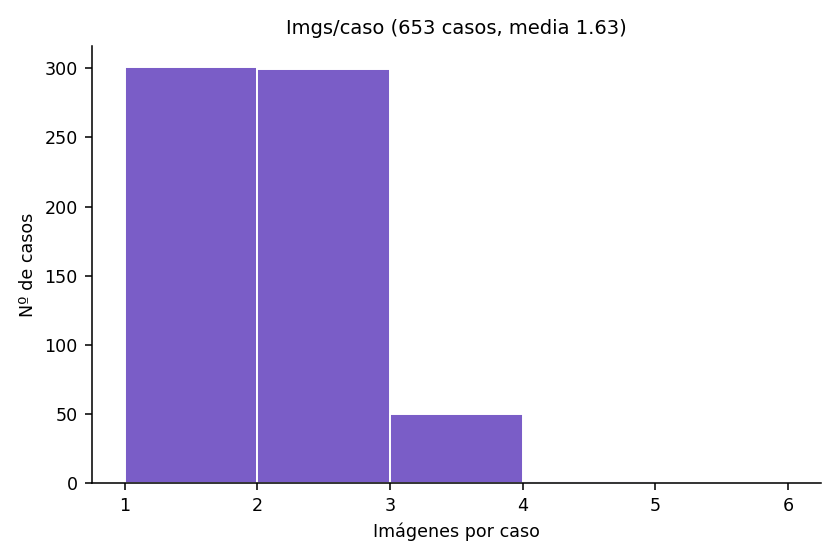
\includegraphics[width=0.85\textwidth]{figures/fig_eda_casos.png}
\caption{Histograma del número de imágenes por caso clínico. La
mayor parte de los casos aportan una o dos imágenes (media
$1{,}63$, mediana $2$, máximo $5$).}
\label{fig:eda-casos}
\end{figure}

\section{Texto narrativo asociado al caso}
\label{sec:anexo-texto}

Cada caso lleva asociado un campo de texto narrativo en castellano
(\texttt{case\_text}) que reproduce, abreviada, la historia clínica
publicada en el blog: motivo de consulta, antecedentes, evolución
temporal y, en ocasiones, el razonamiento diagnóstico inicial. La
longitud mediana del texto es de 223 palabras por caso, con
cuartiles primero y tercero en 175 y 271 palabras respectivamente.
La extensión es relativamente homogénea en el dataset.

Un subconjunto reducido de casos contiene en el texto narrativo la
palabra ``diagnóstico'' o ``diagnosticar'' en construcciones que
podrían anticipar el resultado diagnóstico final: 32 casos
(4,6\% del dataset). Este número es bajo en términos relativos
pero suficiente para justificar la exclusión de estos casos en
escenarios de evaluación zero-shot textual donde el modelo recibe
el \texttt{case\_text} como entrada.

\section{Validación experta y campos de calidad}
\label{sec:anexo-validacion}

El dataset DermapixelAI 1.0 incorpora tres campos de validación
experta cuya distinción es relevante para la interpretación de las
cifras:

\paragraph{\texttt{label\_source = ontology}} (97,89\% del dataset):
la etiqueta diagnóstica L3 final está mapeada a la ontología
jerárquica validada con revisión experta.

\paragraph{\texttt{diagnosis\_source = expert\_v3}} (98,38\% del
dataset): el razonamiento textual asociado al diagnóstico está
respaldado por la tercera revisión experta de la Dra.~Taberner
sobre el dataset.

\paragraph{\texttt{rosa\_verified = True}} (84,39\% del dataset):
\emph{flag} operativo que indica que la imagen ha pasado por
revisión visual explícita por la Dra.~Taberner como ejemplo
representativo del diagnóstico asignado.

Las tres cifras no son intercambiables y conviene declararlas con
precisión en cualquier comunicación derivada del trabajo. En
particular, la cifra que el TFG defendido y los reportes técnicos
asocian a ``validación experta del dataset'' es la primera
(97,89\%), no la tercera. La figura~\ref{fig:eda-calidad}
representa visualmente la composición de los tres campos.

\begin{figure}[H]
\centering
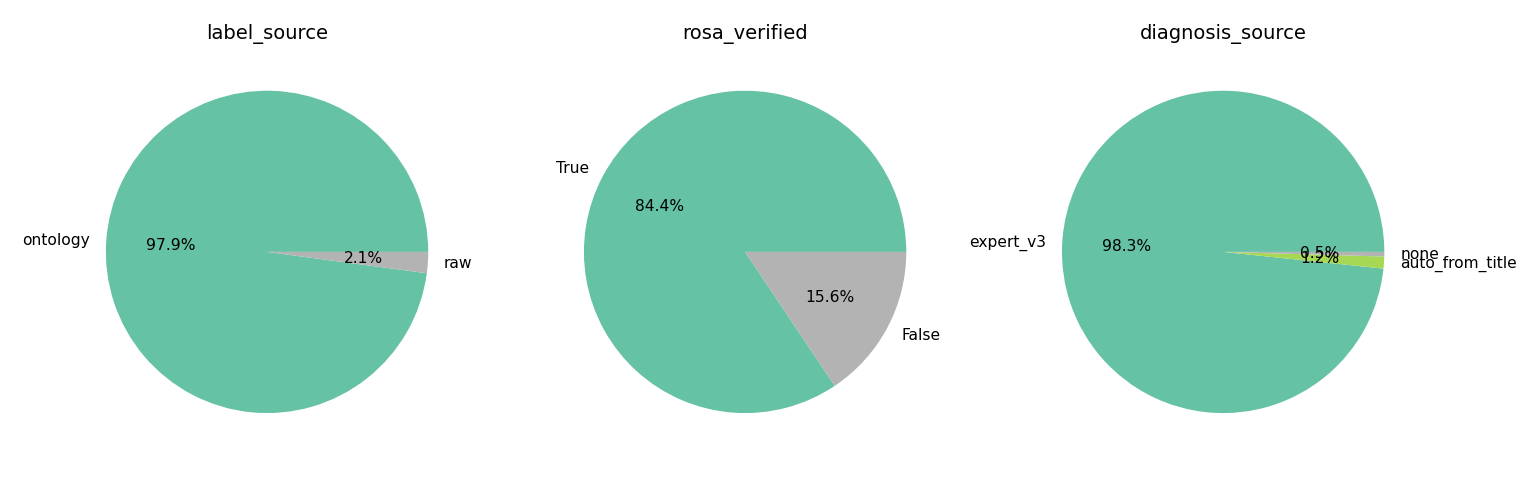
\includegraphics[width=\textwidth]{figures/fig_eda_calidad.png}
\caption{Distribución conjunta de los tres campos de calidad del
dataset DermapixelAI 1.0: \texttt{label\_source},
\texttt{rosa\_verified} y \texttt{diagnosis\_source}. La fracción
con etiqueta L3 mapeada en la ontología ($97{,}89$\%) y la
fracción con razonamiento textual respaldado ($98{,}38$\%)
superan a la fracción operativa con revisión visual explícita
($84{,}39$\%).}
\label{fig:eda-calidad}
\end{figure}

\section{Caracterización temporal y de exclusiones}
\label{sec:anexo-temporal-exclusiones}

\subsection{Distribución temporal}
\label{sec:anexo-temporal}

Las imágenes del dataset DermapixelAI 1.0 se distribuyen en un rango
temporal que abarca desde 2011 hasta 2026, en correspondencia con
los más de quince años de publicación continuada del blog Dermapixel.
La figura~\ref{fig:eda-temporal} muestra la distribución anual de
imágenes incorporadas al dataset. El año de mayor aportación es 2017
con $87$ imágenes; el perfil agregado sugiere una agrupación natural
por décadas (2011--2019 y 2020--2026) que puede emplearse como
estratificación temporal en evaluaciones de robustez frente a cambios
de equipamiento fotográfico o de criterio clínico.

\begin{figure}[H]
\centering
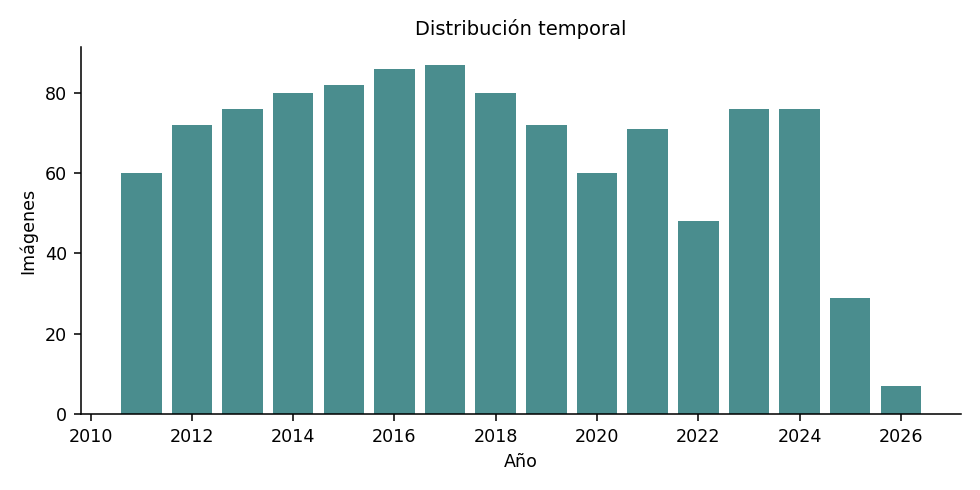
\includegraphics[width=0.85\textwidth]{figures/fig_eda_temporal.png}
\caption{Distribución anual del número de imágenes incorporadas al
dataset DermapixelAI 1.0. Rango $2011$--$2026$; año pico $2017$
con $87$ imágenes.}
\label{fig:eda-temporal}
\end{figure}

\subsection{Razones de exclusión}
\label{sec:anexo-exclusiones}

El pipeline de construcción descartó 80 imágenes del candidato
original. La tabla~\ref{tab:anexo-exclusiones} desagrega las razones
documentadas en \texttt{excluded\_images.csv}.

\begin{table}[H]
\centering
\small
\caption{Razones de exclusión documentadas durante la construcción
del dataset DermapixelAI 1.0.}
\label{tab:anexo-exclusiones}
\begin{tabular}{lr}
\hline
Razón                              & N  \\
\hline
\texttt{not\_found}                & 35 \\
\texttt{not\_derm\_user\_confirmed} & 19 \\
\texttt{md5\_matches\_solution}    & 10 \\
\texttt{dermoscopy\_pending}       & 9  \\
\texttt{dedup\_same\_md5}          & 6  \\
\texttt{not\_derm\_visual\_review} & 1  \\
\hline
\textbf{Total}                     & \textbf{80} \\
\hline
\end{tabular}
\end{table}

La razón más frecuente es \texttt{not\_found} ($35$ imágenes,
correspondientes a páginas del blog no recuperables en la fase de
extracción). Le siguen \texttt{not\_derm\_user\_confirmed} ($19$,
imagen no dermatológica confirmada manualmente),
\texttt{md5\_matches\_solution} ($10$, fuga directa con el panel de
solución del blog, susceptible de inducir \emph{leakage} diagnóstico),
\texttt{dermoscopy\_pending} ($9$, calidad dermatoscópica pendiente
de validación experta), \texttt{dedup\_same\_md5} ($6$, duplicados
exactos) y \texttt{not\_derm\_visual\_review} ($1$, exclusión por
revisión visual posterior). El registro íntegro de exclusiones
permite la reproducción exacta del filtrado y la auditoría de
integridad descrita en el paso (vi) del pipeline.
